% Auteur : Louis de Campou
\begin{frame}{Wormhole}
    Version 1 : \textit{Bridge} entre Ethereum et Solana
    \newline 
    \newline
    Version 2 : Protocole générique de passage de messages qui connecte 22 \textit{blockchains}.
    \newline
    
    \begin{itemize}
        \item Gardiens
        \item VAA (\textit{verified action approval})
        \item \textit{Payloads}
    \end{itemize}
\end{frame}
    
\begin{frame}{Wormhole : Gardiens}
    
    Un gardien est une autorité de confiance qui a comme rôle de valider un message.\newline
    
        \begin{block}{Caractéristiques du réseau de gardiens}
            \begin{itemize}
                \item Sans leader
                \item 19 gardiens à parts égales
                \item Preuve d'autorité (PoA)
                \item \textit{Multisignature} (M/N)
                \item Le consensus est atteint lorsque 2/3 des gardiens ont signé le message
            \end{itemize}
        \end{block}
\end{frame}
    
\begin{frame}{Wormhole : VAA}
    
    Primitive de messagerie de base de Wormhole
    \newline
    
    En-tête :
    \begin{itemize}
        \item Index de l'ensemble des gardiens
        \item Nombre de signatures stockées
        \item Collection des signatures ECSDA (secp256k1)
    \end{itemize}
    
    Corps : 
    \begin{itemize}
        \item L'ID de la chaîne Wormhole du contrat émetteur
        \item L'adresse du contrat émetteur
        \item Le \textit{payload}
    \end{itemize}
\end{frame}
    
\begin{frame}{Wormhole : \textit{Payloads}}
    
    Charges utiles spécifiques attachées à un VAA depuis une chaîne source pour indiquer à la chaîne cible comment traiter le message Wormhole après vérification.\newline
    
    5 payloads au total dont :
    \begin{itemize}
        \item \textit{AssetMeta} : informe des méta-données de l'actif verrouillé, obligatoire avant un premier transfert
        \item \textit{Transfer} : déclenche la libération de jetons verrouillés
    \end{itemize}
\end{frame}
    
\begin{frame}{Wormhole : Architecture simplifiée}
    \centering
    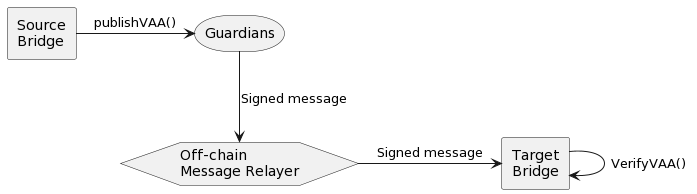
\includegraphics[scale = 0.5]{centralisation/wormhole_louis.png}
\end{frame}
    
\begin{frame}{Wormhole : Récapitulatif}
    \begin{block}{Avantages}
        \begin{itemize}
            \item Un bridge et un protocole important de l'éco-système avec plus de 280M de \$ verrouillés
            \item Rapidité dans le traitement des messages
            \item Scalable

        \end{itemize}
    \end{block}

    \begin{block}{Inconvénients}
        \begin{itemize}
            \item Le réseau de gardiens est l'élement le plus critique mais aussi le plus opaque
            \item Rétablissement d'un modèle de confiance
            \item Justification de sa décentralisation par la présence de plusieurs parties dans le contrôle du réseau
        \end{itemize}
    \end{block}
\end{frame}

% @startuml

% rectangle r1 as "Source
% Bridge"
% storage "Guardians" as r2
% hexagon r3 as "Off-chain 
% Message Relayer" 
% rectangle r4 as "Target
% Bridge"

% r1 -> r2 : publishVAA()
% r2 -do-> r3 : Signed message
% r3 -> r4 : Signed message
% r4 -> r4 : VerifyVAA()

% @enduml
